\documentclass[10pt]{report}
\usepackage[a4paper]{geometry}
\usepackage[myheadings]{fullpage}
\usepackage{fancyhdr}
\usepackage{lastpage}
\usepackage{graphicx, wrapfig, subcaption, setspace, booktabs}
\usepackage[T1]{fontenc}
\usepackage[font=small, labelfont=bf]{caption}
\usepackage{fourier}
\usepackage[protrusion=true, expansion=true]{microtype}
\usepackage[english]{babel}
\usepackage{sectsty}
\usepackage{url, lipsum}
\usepackage{comment}
\graphicspath{ {images/} }

% Setup in line code
% copied from https://tex.stackexchange.com/questions/19004/how-to-format-an-inline-source-code
\usepackage{listings}
\usepackage{color}
\definecolor{lightgray}{gray}{0.9}
\definecolor{dkgreen}{rgb}{0,0.6,0}
\definecolor{mauve}{rgb}{0.58,0,0.82}
\lstset{
    showstringspaces=false,
    basicstyle=\ttfamily,
    keywordstyle=\color{blue},
    commentstyle=\color[grey]{0.6}
    stringstyle=\color[RGB]{255,150,75}
}

\newcommand{\inlinecode}[2]{\colorbox{lightgray}{\lstinline[language=#1]$#2$}}


\newcommand{\HRule}[1]{\rule{\linewidth}{#1}}
\onehalfspacing
\setcounter{tocdepth}{5}
\setcounter{secnumdepth}{5}

% HEADER & FOOTER
\pagestyle{fancy}
\fancyhf{}
\setlength\headheight{15pt}
\fancyhead[L]{Student ID: 1000921236}
\fancyhead[R]{University of Texas at Arlington}
\fancyfoot[R]{Page \thepage\ of \pageref{LastPage}}


% TITLE PAGE
\begin{document}

\title{ \normalsize \textsc{IE 3301 - 004 Honors\\ Engineering Probability}
        \\ [2.0cm]
        \HRule{0.5pt} \\
        \LARGE \textbf{\uppercase{Analysis of UTA Student Feedback Survey Results}} \\
        \normalsize \textit{Part I}
        \HRule{2pt} \\ [0.5cm]
        \normalsize \today \vspace*{5\baselineskip}}

\date{}

\author{
    Joe Cloud \\
        Student ID: 1000921236 \\
        University of Texas at Arlington \\[1in]
        \textit{I, Joe Cloud, did not give or receive any assistance on }\\
        \textit{this project, and the report submitted is wholly my own.}}



    \maketitle
\tableofcontents
\newpage

%-------------------------------------------------------------------------------
% Section title formatting
\sectionfont{\scshape}
%-------------------------------------------------------------------------------

% BODY
\section*{Introduction}
\addcontentsline{toc}{section}{Introduction}


Intro

\section*{Data}
\addcontentsline{toc}{section}{Data}

\subsection*{Set One}
\addcontentsline{toc}{subsection}{Set One}

Data collection began with the process of measuring the resistance of each resistor
and recording its value. The measurements were conducted with a calibrated 4.5 digit
digital multimeter (see Appendix V for equipment information). To perform this measurement,
a digital multimeter was placed in 'resistance' measuring mode, and with probes attached to the correct ports, 
each resistor was attached to the end of the probe on either side of the filament. Once attached the resistive value 
would be flashed on the display of the digital multimeter. Each measurement was entered
into a spreadsheet and later outputed to a CSV file for further processing by data analysis scripts. \\
Before data analysis was performed, $0.33\Omega$ was subtracted from each value, this is done to account
for the resistance added by the multimeter probes. Although this minor offset did not impact the
distribution of measurements for the purposes of the project, it did provide us with results that more 
accurately represent the true values. The values are offset by approximately 0.03\%.

In an ideal world, the resistors would measure identically to the 1k$\Omega$ label.
In reality, the cost to refine manufacturing to attain such level of accuracy is expensive.
Tolerances guarantee a range of possible [random] values which are acceptable for most 
electronics. This dataset was created to explore the distribution of these values.

\subsection*{Set Two}
\addcontentsline{toc}{subsection}{Set Two}
\par
The data collection for Set Two revolved around login access to a compute cluster
and will be difficult to replicate without access to a system with comprehensive logging and login activity.
Though, it is possible for the reader to perform similar analysis with data from a personal machine's logged data. 
On a Unix-like operating system this can be performed with the use of the \inlinecode{Bash}{last} command. 
One of the benefits of computer-triggered collection is that it is much less susceptible to timing errors 
as opposed to that of a 'human polling' based approach. \\ I included the source code necessary to collect 
the data in Appendix IV.C. The process is largely computational. After the raw data was collected with the
\inlinecode{Bash}{last} command, the data was parsed through a preprocessing script written to convert the 
timestamps in HH:MM:SS format to that of total seconds. Then, each event was subtracted from the next, yielding 
interlogin times. The negative sign is discarded as only the magnitude is significant.
As a side note, all source code written for this project are included in the appendix.

\newpage

% Data analysis
\section*{Descriptive Analysis}
\addcontentsline{toc}{section}{Descriptive Analysis}

This section details the results of analysis performed on both datasets One and Two.
To analyze the data, python scripts were written to perform the requested calculations and output the desired
plots for each dataset. The scripts are included as part of the Code section of Appendix IV.A.

\subsection*{Set One}
\addcontentsline{toc}{subsection}{Set One}

\begin{wrapfigure}{r}{0.50\textwidth}
    \centering
    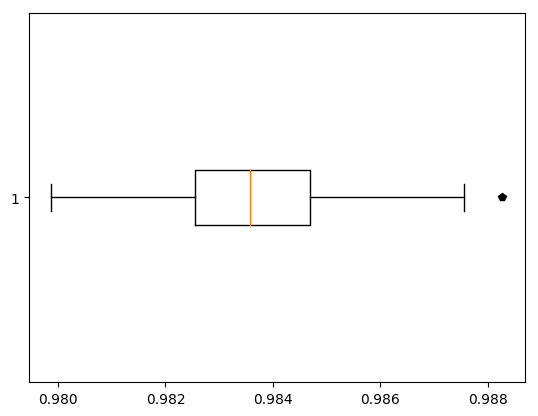
\includegraphics[width=0.50\textwidth]{results/resistor_boxplot}
    \caption{Set One: Box-and-whisker plot}
\end{wrapfigure}

The first step in analysis for Set One was calculating the mean $\bar{X_1}$, which is  $0.98349$ $k\Omega$,
between a minimum value of $0.97987 k\Omega$ and a maximum value of $0.98827 k\Omega$. The next step was calculating
the standard deviation, $\sigma_1$. This was done using \inlinecode{Python}{numpy} as opposed
to doing it by hand with $\sigma_1 = \sqrt{\frac{1}{N-1} \sum_{i=1}^N (X_i - \bar{X_1})^2}$.
The result for $\sigma_1$ was $0.001739$, which would indicate that the spread from the mean is fairly low,
considering the significance of the value.
The last calculation necessary for box-and-whisker plot was the quartiles,
in which $Q1 = 0.98257 k\Omega, Q2 = 0.98659 k\Omega, Q3 = 0.98467 k\Omega$.


The box-and-whisker plot is a helpful method of visualizing spread within a dataset.
The vertical line segments end on either side of the box represent the minimum and maximum
values within the sample space, while the dot to the right represents outliers within the data.
The box itself is useful for showing the quartiles (first being the left edge of the box, with
third being the right).
In this set, the data appears to be dispersed somewhat evenly. The whiskers are similar in length,
with only a slight bias towards the left. This would indicate that the resistant of the 1k$\Omega$
hold an average lower than the median resistance. (x-axis is resistance in k$\Omega$)

\begin{wrapfigure}[14]{r}{0.50\textwidth}
    \centering
    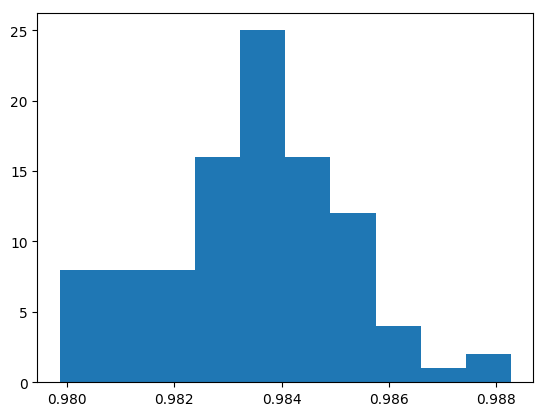
\includegraphics[width=0.50\textwidth]{results/resistor_histogram}
    \caption{Set One: Histogram}
\end{wrapfigure}



The frequency table (Appendix III.A) was created first by determining a bin size. The range of the data was
divided into 10 equal parts. Each bin would contain the tally of the values within
a particular slice. For the resistor values, which is a continuous random variable that we
suspect to be normally distributed, it is promising to see that the tallies peak where the center-most values are located. 
The right-most extreme values do appear to decrease quite significantly, while
the lower end appears to contain more tallies than we would expect for a proper normal distribution.

The histogram represents the distribution of the resistive values across 10 bins, where the y-axis 
is the number of values tallied within the slice, and x-axis is the measured resistance in units of k$\Omega$.
Based on the histogram and previous data analysis, the sample of resistors do not follow a
normal distribution due to a lack of symmetry.



\subsection*{Set Two}
\addcontentsline{toc}{subsection}{Set Two}

The first step in analysis for Set Two was calculating the mean $\bar{X_2}$, which is $8445.05$ seconds (s),
between a minimum value of $1.0$s (restricted by measurement resolution) and a maximum value of $83749$s. 
The next step was calculating the standard deviation, $\sigma_2$, which was $15392.12$s. 
This indicates that spread from the mean is high. The last calculation necessary for box-and-whisker plot was the quartiles,
in which $Q1 = 251.75s, Q2 = 1865.0s, Q3 = 8052.25s$.

\begin{wrapfigure}{r}{0.50\textwidth}
    \centering
    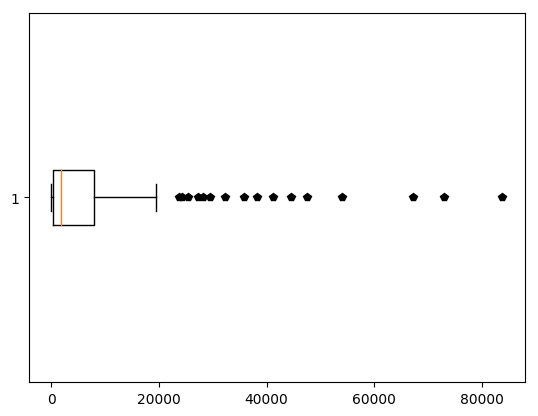
\includegraphics[width=0.50\textwidth]{results/logininterval_boxplot}
    \caption{Set Two: Box-and-whisker plot}
\end{wrapfigure}

In this set, the data appears to be heavily right skewed, with the majority of the values located on the lower
end of the scale (in seconds) and a few large outliers to the right. This foreshadows an interesting frequency
distribution and histogram. Since this interval data is extracted from timestamps, we suspect the data to follow an
exponential distribution. It is based on a continuous random variable (through the time stamp), but the values are
discretized due to the limits of logging precision.

\begin{wrapfigure}[11]{r}{0.50\textwidth}
    \centering
    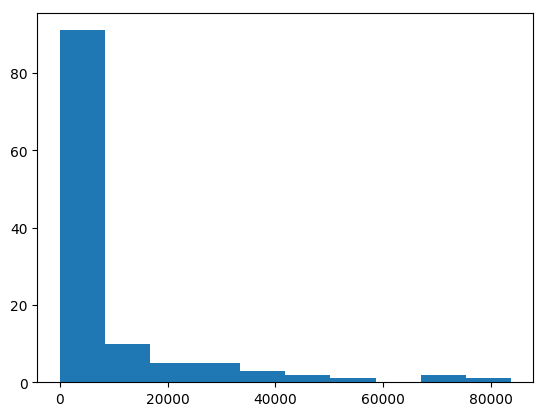
\includegraphics[width=0.50\textwidth]{results/logininterval_histogram}
    \caption{Set Two: Histogram}
\end{wrapfigure}

Similar to Set One, the frequency table (Appendix III.B) was created first by determining a bin size. The range of the data was
divided into 10 equal parts as well. Each bin contained the tally of the values within a particular slice.
When tabled, the values for the login intervals showed that the vast majority
of tallies were entered into the first slice, and a significant decrease in each successive step. The second
through the last bin combined makes up less than a third of the tallies of the first bin.


The histogram to the right represents the distribution of the login interval values across 10 bins.
Where the y-axis is the number of values tallied within the slice, and x-axis is time between successive logins
in seconds.
Based on the histogram and previous data analysis, I conclude that the data follows an exponential distribution. As
interval increases there is an exponential decrease in the values recorded, with some outliers to the extreme but 
with more samples the overall distribution would continue to show strong resemblance to that of the standard
exponential distribution.


\newpage
\section*{Appendix}
\addcontentsline{toc}{section}{Appendix}

\subsection*{I - Dataset: One}
\addcontentsline{toc}{subsection}{I - Dataset: One}

Measured resistance of each resistor in the batch of 100.


\begin{tabular}{rrrrrrrrrr}
    \hline
     0.98227 & 0.98467 & 0.98377 & 0.98277 & 0.97987 & 0.98467 & 0.98437 & 0.98337 & 0.98317 & 0.98507 \\
      0.98027 & 0.98077 & 0.98487 & 0.98037 & 0.98457 & 0.98237 & 0.98387 & 0.98367 & 0.98257 & 0.98487 \\
       0.98377 & 0.98217 & 0.98017 & 0.98487 & 0.98447 & 0.98737 & 0.98317 & 0.98287 & 0.98477 & 0.98417 \\
        0.98207 & 0.98387 & 0.98757 & 0.98427 & 0.98477 & 0.98257 & 0.98537 & 0.98517 & 0.98037 & 0.98007 \\
         0.98527 & 0.98617 & 0.98397 & 0.98127 & 0.98357 & 0.98367 & 0.98387 & 0.98097 & 0.98357 & 0.98077 \\
          0.98287 & 0.98087 & 0.98627 & 0.98107 & 0.98377 & 0.98327 & 0.98537 & 0.98357 & 0.98577 & 0.98547 \\
           0.98247 & 0.98507 & 0.98337 & 0.98367 & 0.98527 & 0.98347 & 0.98827 & 0.98207 & 0.98337 & 0.98297 \\
            0.98297 & 0.98097 & 0.98387 & 0.98287 & 0.98467 & 0.98327 & 0.98157 & 0.98037 & 0.98487 & 0.98117 \\
             0.98547 & 0.98397 & 0.98437 & 0.98337 & 0.98317 & 0.98287 & 0.98507 & 0.98397 & 0.98287 & 0.98327 \\
              0.98167 & 0.98197 & 0.98317 & 0.98547 & 0.98377 & 0.98637 & 0.98057 & 0.98277 & 0.98547 & 0.98447 \\
              \hline
\end{tabular}

% insert table of resistor values here

\subsection*{II - Dataset: Two}
\addcontentsline{toc}{subsection}{II - Dataset: Two}
% insert table of login time values

The interlogin time for users on the compute cluster, in seconds. 120 interlogin times recorded.

\begin{tabular}{rrrrrrrrrrrr}
    \hline
    1796 & 67183 &  7901 & 13437 &  6645 &   916 & 41159 &  8269 &  2684 & 38237 & 3263 & 47470 \\
    6397 & 24371 & 28258 & 12257 &  1348 & 18621 &  6675 &  2691 & 25385 &    86 &   10 & 18647 \\
    68 &    31 &    19 &  2202 &   124 &   508 &     3 & 72894 &  5630 & 15758 & 7980 &   431 \\
    3918 &  3541 & 11982 & 35755 &  6654 &  2526 & 15853 &  3533 &   507 &   367 & 1404 &  2306 \\
    2237 & 23714 &   887 &   141 &  5493 &   520 & 83749 &  3516 & 29573 & 27200 &    2 & 32295 \\
    2197 &  3579 &  4556 &   166 &   864 &    56 &   113 &    98 &     5 &  1645 &    3 &  7368 \\
    1846 &  2136 &  2214 &   213 &   535 &   632 &  1440 &   268 &   243 &   303 & 1182 & 54091 \\
    1 & 19565 &   690 &   243 &    83 &   135 &    84 &  3346 &  6641 &  1373 &  457 &   393 \\
    19 &   187 &   376 &  9292 &  1214 &   589 &   567 &  1240 &  1884 &   207 &  423 &     5 \\
    905 & 44505 &    71 & 11948 & 10404 &  2151 &  2413 &   227 & 10287 &   196 &   25 &  8480 \\
    \hline
\end{tabular}


\subsection*{III - Tables}
\addcontentsline{toc}{subsection}{III - Tables}

\subsubsection*{A - Set One: Frequency table}
\addcontentsline{toc}{subsubsection}{A - Set One: Frequency table}

\begin{table}[h!]
    \centering

    \begin{tabular}{ | l | c | }
        \hline
        Value Range & Count \\
        \hline
        $0.97987 \leq X < 0.98071$ & 8  \\
        $0.98071 \leq X < 0.98155$ & 8  \\
        $0.98155 \leq X < 0.98239$ & 8  \\
        $0.98239 \leq X < 0.98407$ & 16 \\
        $0.98407 \leq X < 0.98491$ & 25 \\
        $0.98491 \leq X < 0.98575$ & 17 \\
        $0.98575 \leq X < 0.98659$ & 12 \\
        $0.98659 \leq X < 0.98743$ & 4  \\
        $0.98473 \leq X < 0.98827$ & 1  \\
        $0.98827 \leq X$           & 2  \\
        \hline
    \end{tabular}
    \caption{Set One: Frequency table}
\end{table}



\subsubsection*{B - Set Two: Frequency table}
\addcontentsline{toc}{subsubsection}{B - Set Two: Frequency table}

\begin{table}[h!]
    \centering

    \begin{tabular}{ | l | c | }
        \hline
        Value Range & Count \\
        \hline
        $1.00000 \leq X < 8375.00$ & 91 \\
        $8375.00 \leq X < 16750.0$ & 10 \\
        $16750.0 \leq X < 25125.4$ & 5  \\
        $25125.4 \leq X < 33500.2$ & 5  \\
        $33500.2 \leq X < 41875.0$ & 3  \\
        $41875.0 \leq X < 50249.8$ & 2  \\
        $50249.8 \leq X < 58624.6$ & 1  \\
        $58624.6 \leq X < 66999.4$ & 0  \\
        $66999.4 \leq X < 75374.2$ & 2  \\
        $75374.2 \leq X$           & 1  \\
        \hline
    \end{tabular}
    \caption{Set Two: Frequency table}
\end{table}


\subsection*{IV - Code}
\addcontentsline{toc}{subsection}{IV - Code}


\subsubsection*{A - Descriptive Analysis}
\addcontentsline{toc}{subsubsection}{A - Descriptive Analysis}


\lstset{frame=tb,
  language=Python,
  aboveskip=3mm,
  belowskip=3mm,
  showstringspaces=false,
  columns=flexible,
  basicstyle={\small\ttfamily},
  numbers=none,
  numberstyle=\tiny\color{gray},
  keywordstyle=\color{blue},
  commentstyle=\color{dkgreen},
  stringstyle=\color{mauve},
  breaklines=true,
  breakatwhitespace=true,
  tabsize=3
}

\begin{lstlisting}
#AUTHOR: Joe Cloud
#PURPOSE: Perform simple descriptive analysis for Probability & Statistics for Engineers, project
#UTA FALL 2017


import numpy as np
import sys
import matplotlib.pyplot as plt
import tabulate

DATA_FILE = "../set_one/resistor_vals_offset.csv"  # Set to default list
QUARTILES = [25, 50, 75]

if len(sys.argv) > 1:
    DATA_FILE = sys.argv[1]

OUTPUT_FILE = "results/" + DATA_FILE.split('/')[-1].split('vals')[0]


def main():

    sample_vals = np.genfromtxt(DATA_FILE, delimiter=',')
    print(sample_vals)

    print("Min value is: %f" % min(sample_vals))
    print("Max value is: %f" % max(sample_vals))

    sample_mean = np.mean(sample_vals)
    print("Mean value is: %f" % sample_mean)

    sample_std = np.std(sample_vals)
    print("STD value is: %f" % sample_std)

    # Calculate quartiles
    sample_quarts = []
    for quart in QUARTILES:
        sample_quarts.append(np.percentile(sample_vals, quart))

    print("Quartiles: ", *sample_quarts, sep=', ')

    generateTable(sample_vals)

    # Construct box-and-whisker plot, a.k.a. boxplot
    fig = plt.figure()
    ax = plt.subplot(111)
    ax.boxplot(sample_vals, 0, 'kp', 0)
    fig.savefig(OUTPUT_FILE + 'boxplot.png', bbox_inches='tight')
    fig.clf()

    num_bins = 10

    # Frequency table
    frequency_table = np.histogram(sample_vals, bins=num_bins)
    print(frequency_table)

    # Histogram data
    fig = plt.figure()
    ax = plt.subplot(111)
    ax.hist(sample_vals, bins=num_bins)
    fig.savefig(OUTPUT_FILE + 'histogram.png', bbox_inches='tight')
    fig.clf()


def generateTable(data):

    data_c = data.reshape(10, int(len(data)/10))
    print(data_c.shape)

    gen_table = tabulate.tabulate(data_c, tablefmt="latex")
    print(gen_table)

    outfile = open(OUTPUT_FILE + 'latex_gen.txt', 'w')
    outfile.write("\n\n\n")
    outfile.write("%s\n" % gen_table)


if __name__ == "__main__":
    main()
\end{lstlisting}



\subsubsection*{B - Data Processing: Set One}
\addcontentsline{toc}{subsubsection}{B - Data Processing: Set One}

\begin{lstlisting}

#!/usr/bin/env python3

# This simply offsets each value by 0.33

FILE_NAME="resistor_vals.csv"

def main():

    f = open(FILE_NAME, 'r')

    data = f.readlines()

    print(data)

    data_output = []
    for val in data:
        data_output.append(float(val) - 0.00033)

    outfile = open("resistor_vals_offset.csv", 'w')

    for val in data_output:
        outfile.write("%s\n" % val)


if __name__ == "__main__":
    main()

\end{lstlisting}

\subsubsection*{C - Data Processing: Set Two}
\addcontentsline{toc}{subsubsection}{C - Data Processing: Set Two}

\begin{lstlisting}

#!/usr/bin/env python3

# This performs necessary pre-processing for raw data from 'last' command

FILE_NAME = "stripped_batch_three.log"

def main():

    f = open(FILE_NAME, 'r')
    data = f.readlines()
    data_conved = convToSeconds(data)
    print(data_conved)
    data_interval = calcInterval(data_conved)
    print(data_interval)

    outfile = open("logininterval_vals.txt", 'w')

    for val in data_interval:
        outfile.write("%s\n" % val)


def convToSeconds(data):

    in_seconds = []

    for login in data:
        # Takes value in format HH:MM:SS and tokenizes, adds up each delimited element
        # w/ respective multiplier.
        temp_tok = login.split(':')

        in_seconds.append(int(temp_tok[2])+int(temp_tok[1])*60+int(temp_tok[0])*3600)

    return in_seconds


def calcInterval(data):
    in_intervals = []
    # Go through and get the difference between T1 and TO to determine login intervals
    # Must abs values bc for ex, TO may be 23:34:46 and T1 00:12:49 where the difference would be negative
    for i in range(0, len(data) - 1):
        in_intervals.append(abs(data[i] - data[i+1]))

    return in_intervals


if __name__ == "__main__":
    main()


\end{lstlisting}




\lstset{language=Bash}

\begin{lstlisting}

#!/usr/bin/env bash

last -Fwx > last_batch_$1.log
cat last_batch_$1 | awk '{ print $7 }' > stripped_batch_$1.txt

\end{lstlisting}



\subsection*{V - Equipment Used}
\addcontentsline{toc}{subsection}{V - Equipment Used}

\begin{figure}[h!]
    \centering
    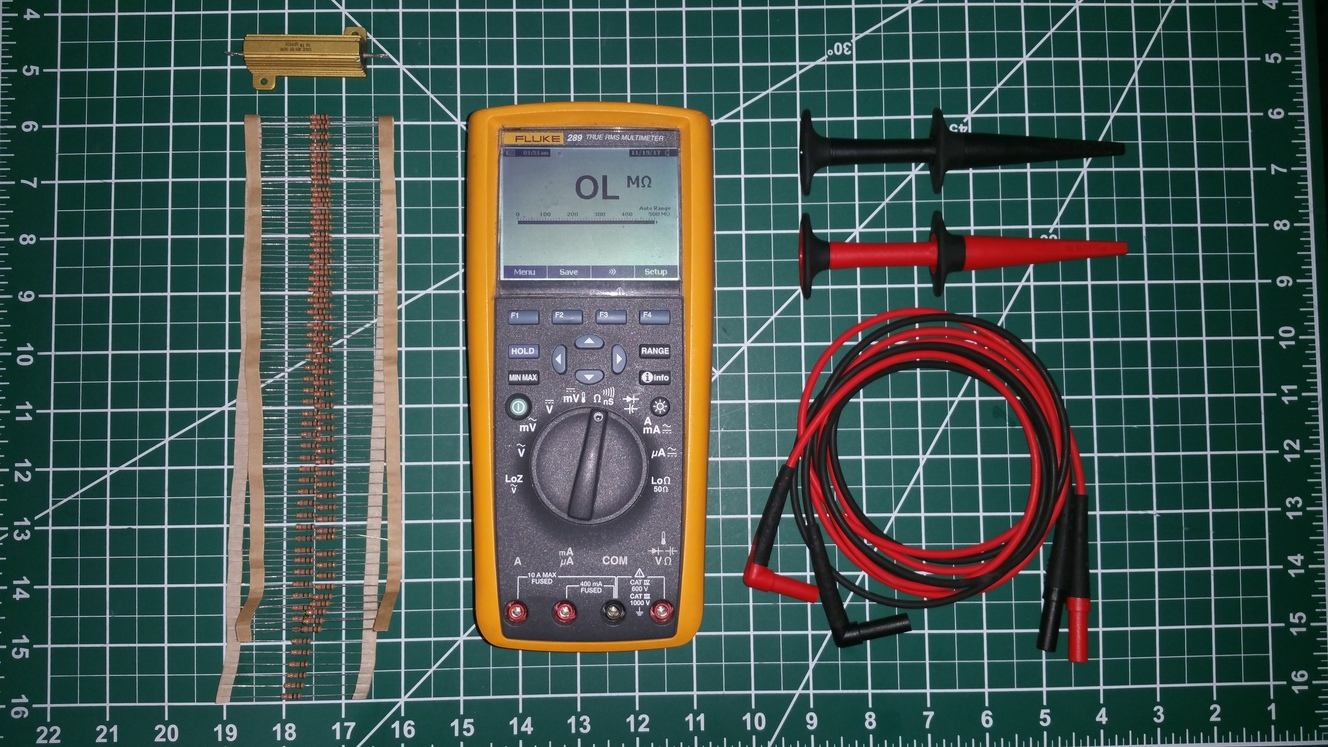
\includegraphics[width=0.7\textwidth]{process/dmm_resistors}
    \caption{Set One: Fluke 289 w/ resistors}
\end{figure}




\begin{comment}
    Report requirements:
    - Define all notation
    - Include descriptions of tables, figures

    Includes:
    - Cover page
    - - Complete, includes nec. info
    - Data section
    - - Describe data collection process
    - - - Enough info for someone to replicate process
    - Descriptive Statistics
    - - Include results from descriptive analysis
    - - Interpret results of:
    - - - Box-and-whisker plot
    - - - Histogram
    - - Do sets follow distributions? 1/2 = normal/exponential dist?
    - Appendices I/II:
    - - Tables of raw data for each set
    - - Code
    - - Equipment used

    Structure:
    - cover
    - table of contents
    - body
    - - motivation
    - - the data
    - - collection process
    - - descriptive statistics
    - - methodologies
    - - - tech used (reference appendece for code/tech used)
    - - results
    - - - figs
    - - answer questions
    - appendices
    - - 1 - set 1 data
    - - 2 - set 2 data
    - - 3 - main analysis code
    - - 4 - helper / preprocessing
    - - 5 - table of equipment

\end{comment}



% REFERENCES
\newpage
\section*{References}
\addcontentsline{toc}{section}{References}

Walpole, R.E., 2016. \textit{Probability and Statistics for Engineers and Scientists}. Prentice Hall.
\newline
\newline


\end{document}
